\documentclass{beamer}

\usepackage[utf8]{inputenc} \usepackage{bibentry,cite,amsmath,graphicx}

\newcommand{\Z}{\mathbb{Z}} \newcommand{\N}{\mathbb{N}}
\newcommand{\R}{\mathbb{R}} \newcommand{\E}{\operatorname{E}}
\newcommand{\Var}{\operatorname{Var}} \newcommand{\Cov}{\operatorname{Cov}}
\newtheorem{proposition}{proposition}
% Information to be included in the title page:
\title{The Kalman-Bucy Filter} \author{Alexander Wittmond} \institute{University of
  Missouri} \date{\today}

\AtBeginSection[] {
  \begin{frame}
    \frametitle{Table of Contents}
    \tableofcontents[currentsection]
  \end{frame}
}

\usetheme{Hannover} \allowdisplaybreaks
\begin{document}

\frame{\titlepage}

\section{The Filtering Problem}

\begin{frame}{Classical Models}

  Classically, time dependent systems are modeled by:
  \pause
  Differential equations 
    \begin{align}
      f &: \R^n \times \R \to \R^n \\
      \frac{dx}{dt} &= f(x,t)
    \end{align}
  \pause
  Solved by:
  \begin{align}
    x : \R \to \R^n
  \end{align}
\end{frame}

\begin{frame}{The problem of noise}
  \begin{itemize}
  \item reality is more complex \pause
  \item measurements of a system have a maximum resolution \pause
  \item beyond that resolution we see random noise caused by unknown variables
    \pause
  \item so our observations are better modeled by a random variable $X$ on some
    probability space $(\Omega,P)$ than a point in $\R^n$
  \end{itemize}

  \begin{figure}
    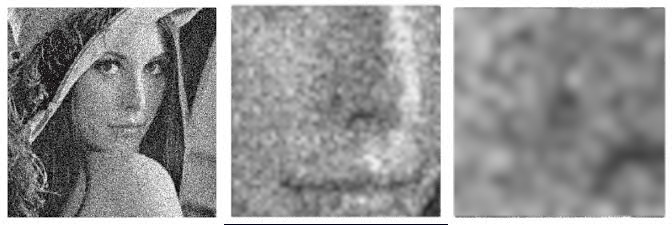
\includegraphics{noise_example}
    \caption{An example of a noisy measurement}
  \end{figure}
\end{frame}

\begin{frame}{Stochastic Models}

    \pause
    Stochastic differential equations
    \begin{align}
      dx_t = f(x_t,t) dt + g(x_t,t) d\beta_t
    \end{align}

    meaning

    \begin{align}
      x_t - x_0 = \int_0^tf(x_t,t) dt + \int_0^tg(x_t,t) d\beta_t
    \end{align}
    \pause
    Solved by a stochastic process

    \begin{align}
      X &: (\Omega,P) \times \R \to \R^n \\
      \{X_t &\}_{t\in R} 
    \end{align}
  


\end{frame}

\begin{frame}{Stochastic Model of Measurement}
  In general we cannot measure a system directly and our measurement may be
  subject to noise.

  \pause

  \begin{align}
    dx_t &= f(x_t,t) dt + g(x_t,t) d\beta_t \\
    y_n  &= h(x_t) + \nu_n
  \end{align}
  \pause We will assume our measurement is subject to white noise
  \begin{equation}
    v_n \sim N(0,R_k) \text{ i.i.d}
  \end{equation}
\end{frame}

\begin{frame}{The Filtering Problem and its Solution}
  Given a set of observations $\{Y_{t_1},\dots,Y_{t_n}\} = Y_{n}$ we want to
  estimate the distribution of $X_t$.

  \pause
  \begin{itemize}
    \pause
  \item \textbf{Smoothing} $t < t_n$ \pause
  \item \textbf{Filtering} $t = t_n$ \pause
  \item \textbf{Prediction} $t > t_n$
  \end{itemize}

  \pause We want to compute
  \begin{equation}
    p(x,t \mid Y_n)
  \end{equation}
  \pause The minimum variance estimate of $X_t$ is
  \begin{equation}
    \mathbb{E}[x \mid Y_t]
  \end{equation}
  the mean of $p(x,t \mid Y_{n})$
\end{frame}

\section{The Kalman-Bucy Filter}

\begin{frame}{The Linear Problem}
  Linear systems are given by:

  \pause
    \begin{align}
      dx_t &= F(t) x_t dt + G(t) d\beta_t \\
      y_k &= M(t_k) x_{t_k} + \nu_k \\
      \mathbb{E}[d\beta_td\beta_t^T] &= Q(t) dt, \quad \nu_k \sim N(0,R_k)
    \end{align}
   \pause
 
\end{frame}

\begin{frame}{Characterization of Linear Systems}
  \begin{itemize}
   
  \item Linear systems are Gauss Markov processes with means described by
    deterministic linear systems.
    \begin{equation}
      x_t \sim N(\hat{x}_t,P_t)
    \end{equation}
   
  \item We only need to know the mean and variance of the system at a given time
    to characterize $P(x,t)$
  \end{itemize}
  \begin{figure}
    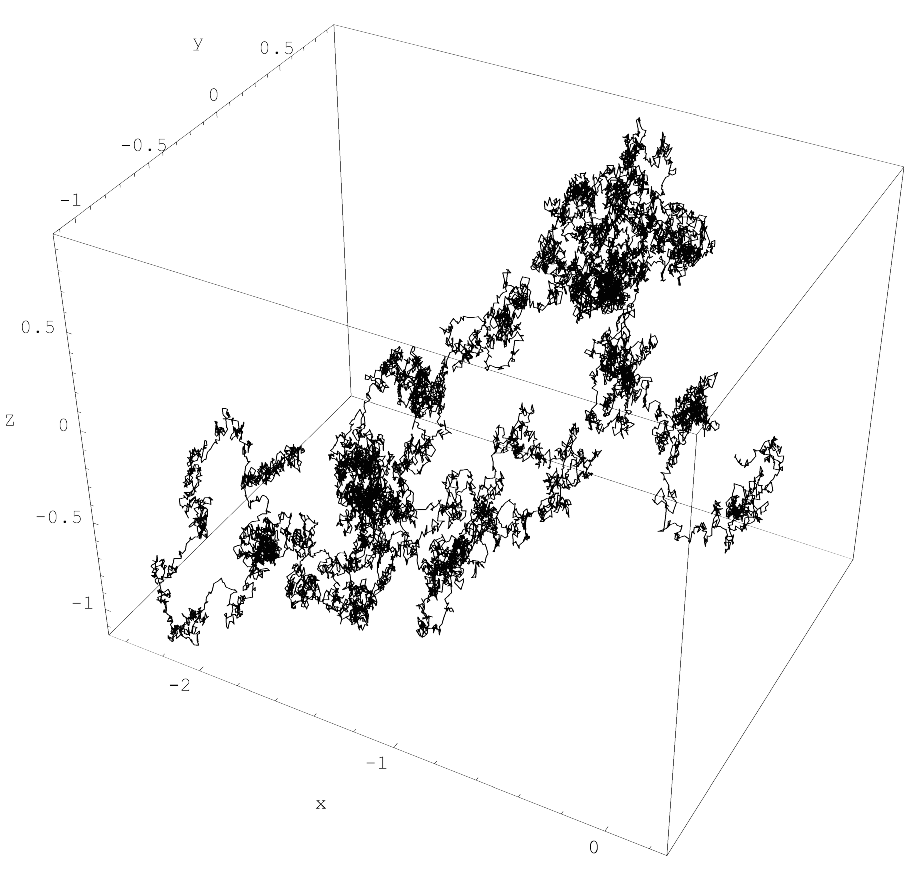
\includegraphics[scale=0.14]{Wiener_process_3d.png}
    \caption{Three dimensional Brownian motion}
  \end{figure}
\end{frame}

\begin{frame}{The Solution To The Linear Discrete-Continuous Filtering Problem}
  The Kalman-Bucy filter consists of: \\
  \only<1>{
    \begin{block}{Evolution for}
      \begin{align}
        \text{Conditional Mean } & \mathbb{E}[x_t \mid Y_{t_k}] = \hat{x} _t^{t_{k}}\\
        \text{Conditional Variance } & \mathbb{E}[(x_t - \hat{x}_t)(x_t - \hat{x}_t)^T \mid Y_{t_k}] = P_t^{t_k}
      \end{align}
      given some prior $x_0$ and $P_0^0$.
    \end{block}
  }
  \only<2>{
    \begin{block}{Prediction between observations}
      \begin{align}
        \frac{d}{dt}{\hat{x}_t^{t_k}} &= F(t)\hat{x}_t^{t_k} \\
        \frac{d}{dt}P^{t_k} &= F(t)P^{t_k}_t +  P^{t_k}_t F^T(t) + G(t)Q(t)G^T(t) \\
        t_k &\leq  t < t_{k+1}
      \end{align}
    \end{block}
  }
  \only<3>{
    \begin{block}{Update at observations}
      \begin{align}
        \hat{x}_{t_k}^{t_k} & = \hat{x}_{t_k}^{t_{k-1}} + K(t_k)(y_k - M(t_k)
        \hat{x}_{t_k}^{t_{k-1}}) \\
          P_{t_k}^{t_{k-1}} &= P_{t_k}^{t_{k-1}} - K(t_k)M(t_k)P^{t_{k-1}}_{t_k}
      \end{align}
      where the \textbf{Kalman Gain} $K(t)$ is given by
      \begin{equation}
        P_{t_k}^{t_{k-1}}M^T(t_k)[M(t_k)P_{t_k}^{t_{k-1}}M^T(t_k) + R_k]^{-1}
      \end{equation}
    \end{block}
  }
\end{frame}

\begin{frame}{In Code}

  \begin{figure}
    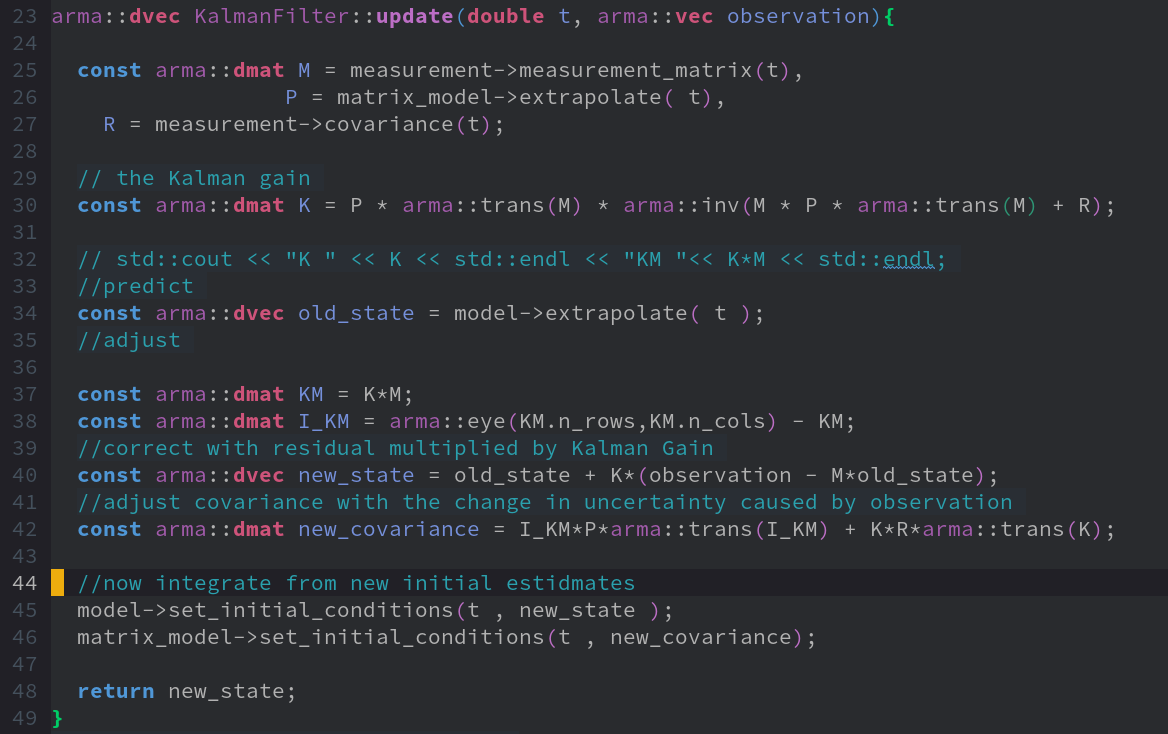
\includegraphics[scale=0.3]{kalman_implementation.png}
    \caption{The Kalman Filter update in C++}
  \end{figure}
\end{frame}

\begin{frame}{Considerations}
  \begin{itemize}
   \pause
\item To integrate the prediction equations we need to fix the boundary
  conditions $\hat{x}_{t_0}$, $P_{t_0}$
   \pause
  \item Calculating the Kalman gain is $O(n^3)$ in the dimension of the
    measurement due to the matrix inversion
    \pause
  \item The Kalman gain can be precomputed
    \pause 
\item The update is recursive so we only need to store our previous estimates at
  the time of the update
 
  \end{itemize}

\end{frame}
 
\begin{frame}{Extension to Non-Linear Problems}
  We start with the system
  \begin{align}
    dx_t = f(x_t,t)dt + G(t)d\beta_t \\
    y_k = h(x_{t_k}, t) + \nu_t
  \end{align}
  where
  \begin{equation}
    \mathbb{E}[d\beta_td\beta^T_t] = Q(t) dt
  \end{equation}
  \pause
  Then we pick a \textbf{reference trajectory} $\bar{x}_{t_0}(t)$ with some given
  $\bar{x}(t_0)$ such that
  \begin{equation}
    \frac{d\bar{x}_{t_0}}{dt}(t) = f(\bar{x}_{t_0}(t),t)
  \end{equation}
\end{frame}

\begin{frame}{Extension to Non-Linear Problems}
  Then we can look at the \textbf{deviation}
  \begin{equation}
    \delta x(t) = x(t) - \bar{x}_{t_0}(t) 
  \end{equation}
  which statisfies
  \pause
  \begin{equation}
    d(\delta x_t) = (f(x_t,t) - f(\bar{x}_{t_0}(t),t)) dt + G(t) d\beta_t
  \end{equation}
  \pause
  then do a Taylor approximation
  \begin{equation}
    f(x_t,t) - f(\bar{x}_t,t) \simeq Df(\bar{x}_{t_0}(t),t)  \delta x_t 
  \end{equation}
  \pause
  Then we have the linear equation
  \begin{equation}
    d(\delta x_t) = Df(\bar{x}_{t_0} , t) \delta x_t dt + G(t) d\beta_t
  \end{equation}
\end{frame}

\begin{frame}{Extension to Non-Linear Problems}
  We can linearize the measurement in the same way to get
  \begin{align}
    \delta y_{t_k} &= y_{t_k} - h(\bar{x}_{t_0}(t_k), t_k) + \nu_k \\
    \delta y_{t_k} &\simeq Dh(\bar{x}_{t_0}(t_k),t_k) \delta x_{t_k} + \nu_k
  \end{align}
  \pause
  Then we can process the system
  \begin{align}
    d(\delta x_t) &= Df(\bar{x}_{t_0}(t),t) \delta x_t dt + G(t) d\beta_t \\
    \delta y_{t_k} & = Dh(\bar{x}_{t_0}(t_k),t_k) \delta x_{t_k} + \nu_k
  \end{align}
  with  linear filter.
\end{frame}

\begin{frame}{Extension to Non-Linear Problems}
  We can then estimate $\hat{x}_{t_k}^{t_k}$ with
  \begin{align}
    \hat{x}_{t_k}^{t_k} = \bar{x}_{t_0}(t_k) + \hat{\delta x_{t_k}^{t_k}}
  \end{align}
  Our variance matrix $P_{t_k}^{t_k}$ estimates the variance of this
  estimation.
\end{frame}

\begin{frame}{Extension to Non-Linear Problems}
  If at every observation $h(t_k)$, we relinearize around our estimate
  $\hat{x}_{t_k}^{t_k}$ by getting a new reference trajectory $\bar{x}_{t_k}(t)$
  starting at this point, and then estimate the system using

  
  \begin{align}
    d(\delta x_t) &= Df(\bar{x}_{t_k}(t),t_k) \delta x_t dt + G(t) d\beta_t \\
    \delta y_{t_{k+1}} &\simeq Dh(\bar{x}_{t_k}(t_k),t_k) \delta x_{t_k} + \nu_k
  \end{align}

  then this is known as the \textbf{Extended Kalman Filter}
\end{frame}

\begin{frame}{In Code}

\begin{figure}
  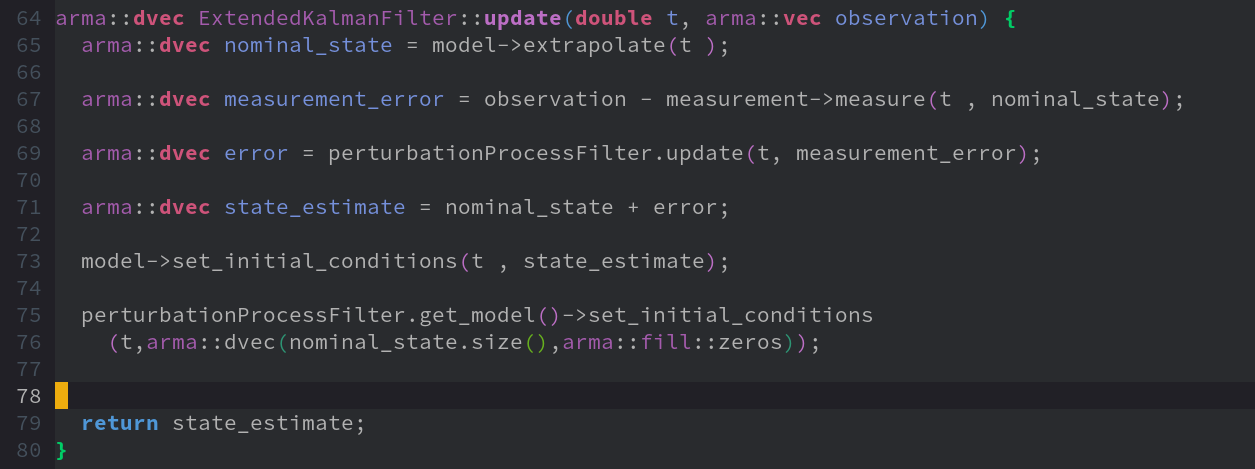
\includegraphics[scale=0.3]{ekf_implementation.png}
  \caption{The Extended Kalman Filter update in C++}

\end{figure}
\end{frame}

\begin{frame}{Pros and Cons}
  \begin{box}{Pros}
    \begin{itemize}
     
    \item Recursiveness causes low memory requirements
     
    \item Relatively low cost to computing an update
     
    \item Most computationally expensive items can be computed in advance

    \end{itemize}
  \end{box}

  \begin{box}{Cons}
    \begin{itemize}

    \item  Is not adaptive, relies on the accuracy of the underlying model

    \item  Can not capture multi-modalities

    \item  Suffers from filter divergence

    \end{itemize}

  \end{box}
\end{frame}
  

\section{An Example}

\begin{frame}{Orbit Determination}
  The simulation will be filtering noisy measurements from a deterministic
  system.

  \pause
  We have
  \begin{align}
    dx_t = f(x_t,t)dt \\
    y_k = h(x_{t_k}, t) + \nu_t\\
    \nu_t \sim N(0,Q) 
  \end{align}

\end{frame}
\begin{frame}{Orbit Determination}
  \begin{equation}
    x_t = \begin{bmatrix}
      x \\
      y \\
      \dot{x} \\
      \dot{y} \\
    \end{bmatrix}
  \end{equation}
  \begin{equation}
    f(x_t,t) = \begin{bmatrix}
      \dot{x} \\
      \dot{y} \\
      - \mu \frac{x}{x^2 + y^2} \\
      - \mu \frac{y}{x^2 + y^2} \\
    \end{bmatrix}
  \end{equation}
\end{frame}

\begin{frame}
  If $p$ gives the position of the sensor and
  \begin{equation}
    \bar{x} = \begin{bmatrix}
      x \\
      y
    \end{bmatrix}
  \end{equation}
  then
  \begin{equation}
    h(x_t,t) = \begin{bmatrix}
      \lVert \bar{x} - p \rVert \\
      \frac{(x - p_1) \dot{x} + (y - p_2) \dot{y}}{\lVert \bar{x} - p \rVert }\\
      \frac{x \cdot p}{\lVert x \rVert}
    \end{bmatrix}
  \end{equation}
  \begin{equation}
    Q_t = \begin{bmatrix}
      n1 & 0 & 0 \\
      0 & n2 & 0 \\
      0 & 0 & n3
  \end{bmatrix}
  \end{equation}
\end{frame}

\begin{frame}
  \begin{figure}
    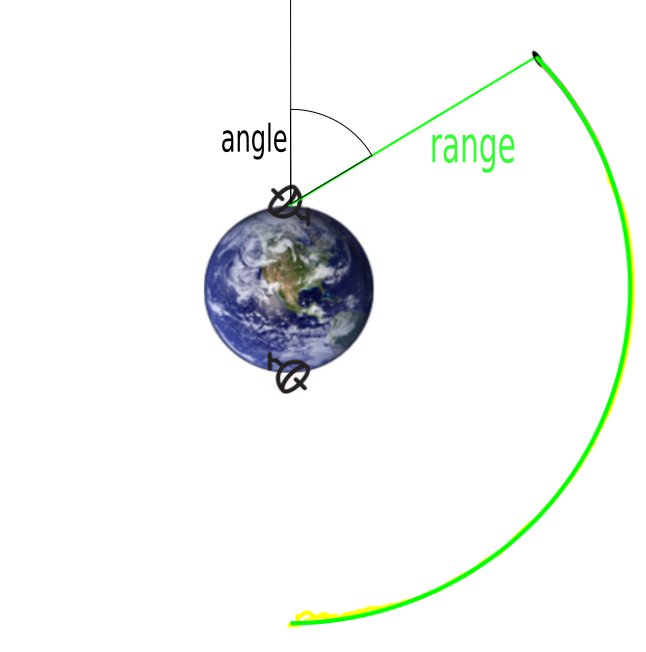
\includegraphics[scale=0.3]{sim_shot.png}
    \caption{Measurements in Simulation}
  \end{figure}

\end{frame}
\end{document}
